\documentclass[a4paper,12pt]{article}
\usepackage[utf8]{inputenc}
\usepackage{hyperref}
\usepackage{listings}
\usepackage{color}
\usepackage{geometry}
\geometry{margin=1in}
\usepackage{amsmath}
\usepackage{graphicx}
\usepackage{amsmath}
\usepackage{hyperref}
\usepackage{setspace}
\usepackage{listings}
\usepackage{xcolor}  % Include xcolor for text color
\usepackage{abstract}
\usepackage{float}
\usepackage{booktabs}
\usepackage{multirow}
\usepackage{siunitx}
\usepackage{caption}
\usepackage{amsmath}
\usepackage{algorithm}
\usepackage{algpseudocode}
\usepackage{hyperref}
\usepackage{tikz}
\usetikzlibrary{positioning}





\title{Embedded control with movement detection: \\ Utilizing MPU9250, MQTT, Node-RED, and InfluxDB and machine learning in esp32.}
\author{Nikolaos Mouzakitis}
\date{May 21, 2025}

\definecolor{codegray}{rgb}{0.5,0.5,0.5}
\definecolor{codepurple}{rgb}{0.58,0,0.82}
\definecolor{backcolour}{rgb}{0.95,0.95,0.92}

\lstdefinestyle{mystyle}{
    backgroundcolor=\color{backcolour},   
    commentstyle=\color{codegray},
    keywordstyle=\color{blue},
    numberstyle=\tiny\color{codegray},
    stringstyle=\color{codepurple},
    basicstyle=\ttfamily\footnotesize,
    breakatwhitespace=false,         
    breaklines=true,                 
    captionpos=b,                    
    keepspaces=true,                 
    numbers=left,                    
    numbersep=5pt,                  
    showspaces=false,                
    showstringspaces=false,
    showtabs=false,                  
    tabsize=2
}

\lstset{style=mystyle}

\begin{document}

\maketitle

\section{Introduction}

This project integrates an ESP32 microcontroller with an MPU9250 
inertial measurement unit (IMU) sensor to detect device movements 
and control 2 LEDs and PWM outputs accordingly. 
It implements a mechanism to persist and restore device state 
via MQTT messaging, Node-RED flow processing, and data storage in an InfluxDB time-series database.

The key 
functionalities are:

\begin{itemize}
    \item Reading accelerometer and gyroscope Y-axis, and magmetometer X-axis data from the MPU9250.
    \item Applying threshold-based logic or machine learning to detect movement and determine LED and PWM states.
    \item Publishing device status data over MQTT.
    \item Restoring device LED and PWM states after reboot using InfluxDB queries and Node-RED.
\end{itemize}


An image of the Esp32 and the MPU sensor used in the project is presented below.
		\begin{figure}[H]
			\centering
			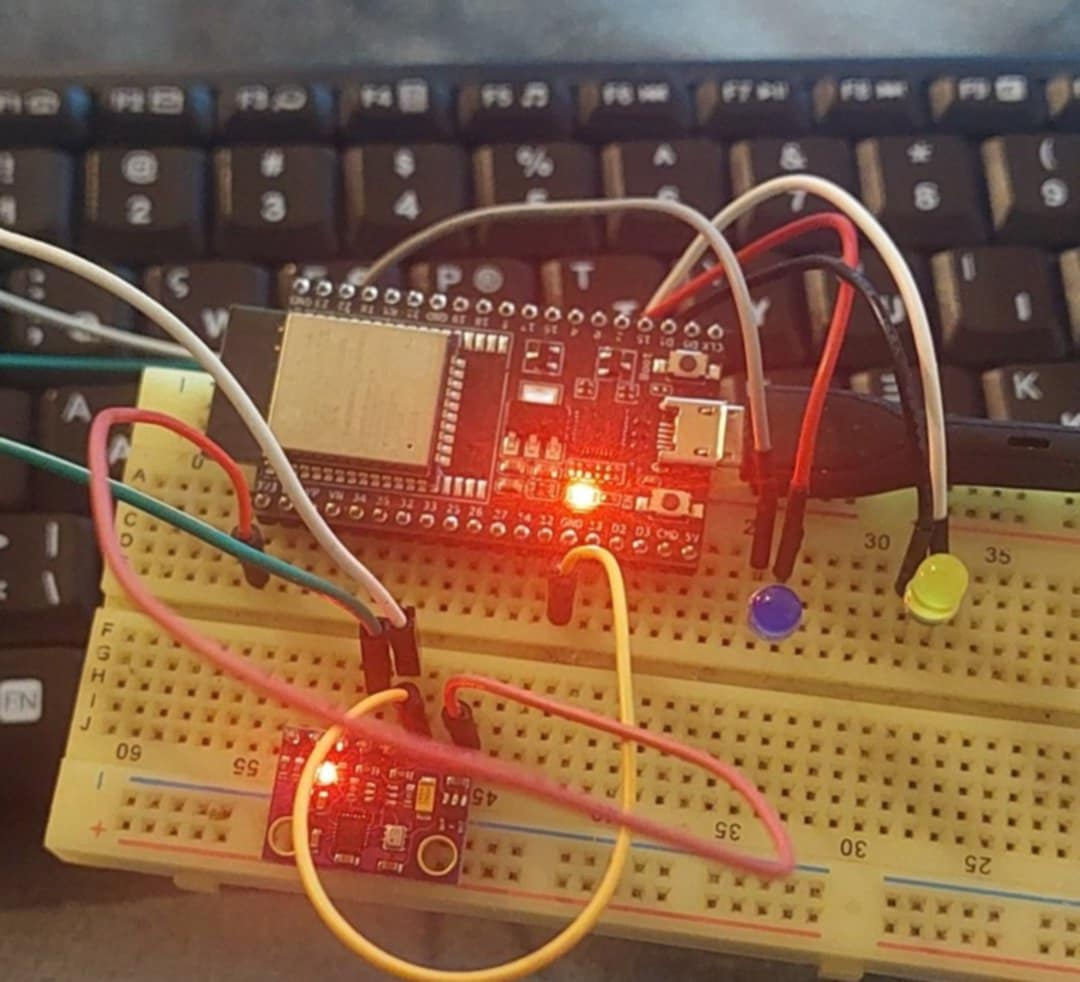
\includegraphics[width=0.5\textwidth]{con.jpeg}
			\caption{esp32 and mpu connected on breadboard.}
			\label{fig1:}
		\end{figure}		




\section{MPU9250 Sensor Data and Movement Detection}

\subsection{Sensor Overview}

The MPU9250 is a 9-axis IMU sensor combining a 3-axis accelerometer, 
3-axis gyroscope, and 3-axis magnetometer. 
For this project, only the accelerometer Y-axis,gyroscope Y-axis and magnetometer X-axis values 
are utilized.
\subsection{Data Acquisition}

The ESP32 reads raw sensor values for accelerometer Y (\texttt{ay}) 
,gyroscope Y (\texttt{gy}) which are used to control the activation of the two LEDs, 
and magnetometer X (\texttt{mx}) which controls the PWM, at periodic intervals.

\subsection{Threshold-Based Movement Detection}

Threshold values are defined empirically to decide when the ESP32 should 
change the states of its LEDs and PWM output.


\subsection{Controlling LEDs and PWM}

Based on movement detection, the device sets the LEDs and a common PWM variable which is applied on 
any LED that is on "active" state.

\subsection{Status Publishing}

The ESP32 publishes its current LED and PWM states 
on the MQTT topic \texttt{esp32/status} as a formatted string:

{\scriptsize
\begin{verbatim}
LED1:OFF LED2:ON PWM:15
\end{verbatim}
}
This message serves to provide the
real-time status of device outputs.

\section{MQTT Communication Architecture}

The ESP32 communicates with the Node-RED 
server via MQTT. Topics used include:

\begin{itemize}
    \item \texttt{esp32/status} — Periodic status updates including LED and PWM states.
    \item \texttt{esp32/restore\_request} — Sent by ESP32 at startup requesting last stored device state.
    \item \texttt{esp32/restore\_state} — Published by Node-RED after querying InfluxDB with the restore state data.
\end{itemize}

\subsection{Restore request and response flow}

Upon powering on, on startup, 
the ESP32 immediately publishes a \texttt{get\_latest} message 
on \texttt{esp32/restore\_request}. 
This triggers Node-RED to query the latest device state 
stored in InfluxDB and respond by publishing a 
formatted restore state message on \texttt{esp32/restore\_state}.

The ESP32 listens for this restore message and 
applies the LED and PWM settings accordingly before 
continuing normal operation.
Restoration can be observed in the following Figure, where the Esp32 
boots and assigns immidiately the latest saved state on the LEDs.

		\begin{figure}[H]
			\centering
			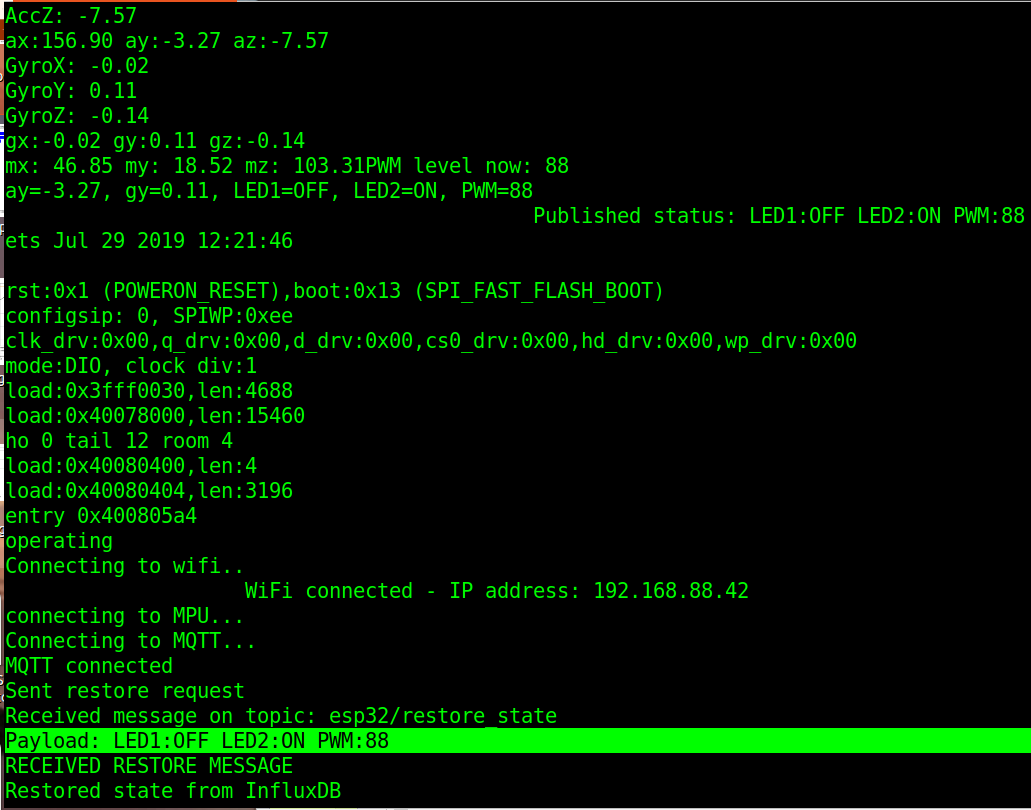
\includegraphics[width=0.9\textwidth]{restore.png}
			\caption{Latest state restoration as observed over UART}
			\label{fig1:}
		\end{figure}		



\section{Node-RED and InfluxDB Integration}

\subsection{Node-RED Flow Design}

Node-RED acts as the middleware for the bridging of MQTT and InfluxDB:

\begin{enumerate}
    \item \textbf{MQTT In node} listens on \texttt{esp32/restore\_request} and 
	    detects the \texttt{get\_latest} message.
    \item \textbf{InfluxDB Query node} performs a time-series query 
	    fetching the most recent LED and PWM state values.
    \item \textbf{Function node} formats the InfluxDB query response 
	    into the MQTT payload string.
    \item \textbf{MQTT Out node} publishes the 
	    formatted message on \texttt{esp32/restore\_state}.
\end{enumerate}


		\begin{figure}[H]
			\centering
			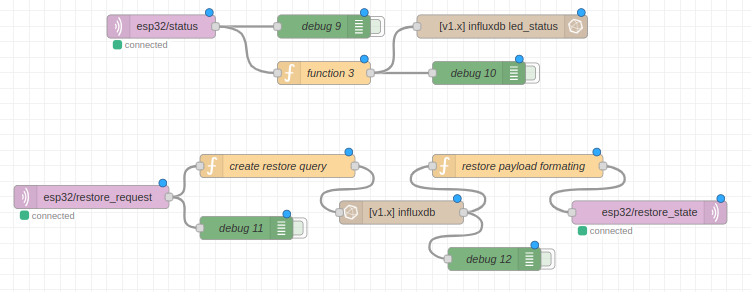
\includegraphics[width=0.9\textwidth]{node1.png}
			\caption{Node-Red data and processing flow}
			\label{fig1:}
		\end{figure}		



\subsection{InfluxDB Query}

As for the InfluxDB, version 1.6.4 has been utilized and installed
as 
{\scriptsize
\begin{verbatim} 
echo "deb https://repos.influxdata.com/ubuntu bionic stable" |  sudo tee /etc/apt/sources.list.d/influxdb.list
sudo curl -sL https://repos.influxdata.com/influxdb.key | sudo apt-key add -
sudo apt get update
sudo apt-get install -y influxdb
\end{verbatim}
}
After installation, a database is created to be used for this project.

{\scriptsize
\begin{verbatim}
influx
> create database esp32db
\end{verbatim}
}

In \texttt{function3} of the Node-Red then, when run the following 
Javascript code in order to push data in the same database.

{\scriptsize
\begin{verbatim}
let parts = msg.payload.split(" ");
let led1 = parts[0].split(":")[1] === "ON" ? 1 : 0;
let led2 = parts[1].split(":")[1] === "ON" ? 1 : 0;
let pwm = parseInt(parts[2].split(":")[1]);

msg.payload = {
    LED1: led1,
    LED2: led2,
    PWM: pwm
};
msg.measurement = "led_status";
return msg;
\end{verbatim}
}

On the InfluxDb out node in Node-Red is also specified and set
the measurement's name as "led\_status" and 
on the server configuration the
respective host ip, port number and database name as "esp32db".



The InfluxDB query used in \texttt{create\_restore\_query} node is:

{\scriptsize
\begin{verbatim}
msg.query = 'SELECT LAST("LED1"), LAST("LED2"), LAST("PWM") FROM "led_status"';
return msg;
\end{verbatim}
}
This query retrieves the most recent LED1, LED2, and PWM values stored.

In the \texttt{restore payload formating} node of Node-Red
response if formated to be given as an input on the \texttt{restore\_state} topic as:

{\scriptsize
\begin{verbatim}
let row = msg.payload[0]; // first row of result

let LED1 = row.last === 1 ? "ON" : "OFF";
let LED2 = row.last_1 === 1 ? "ON" : "OFF";
let PWM = row.last_2;

msg.payload = `LED1:${LED1} LED2:${LED2} PWM:${PWM}`;
msg.topic = "esp32/restore_state";
return msg;
\end{verbatim}
}

\subsection{State Restoration}

Upon receiving the restore payload, the ESP32 parses the string and applies the saved LED and PWM states, 
ensuring the desired recovery.


\subsection{UI visualization}

For the UI visualization 2 switches reflecting the current state of LED have been employed 
and a slider for representing the common PWM applied to them.

A new function named \texttt{function4} have been used to do the same operation as 
\texttt{function3} with the difference of returning3 outputs, one by one to be passed
on the switches and the slider.


		\begin{figure}[H]
			\centering
			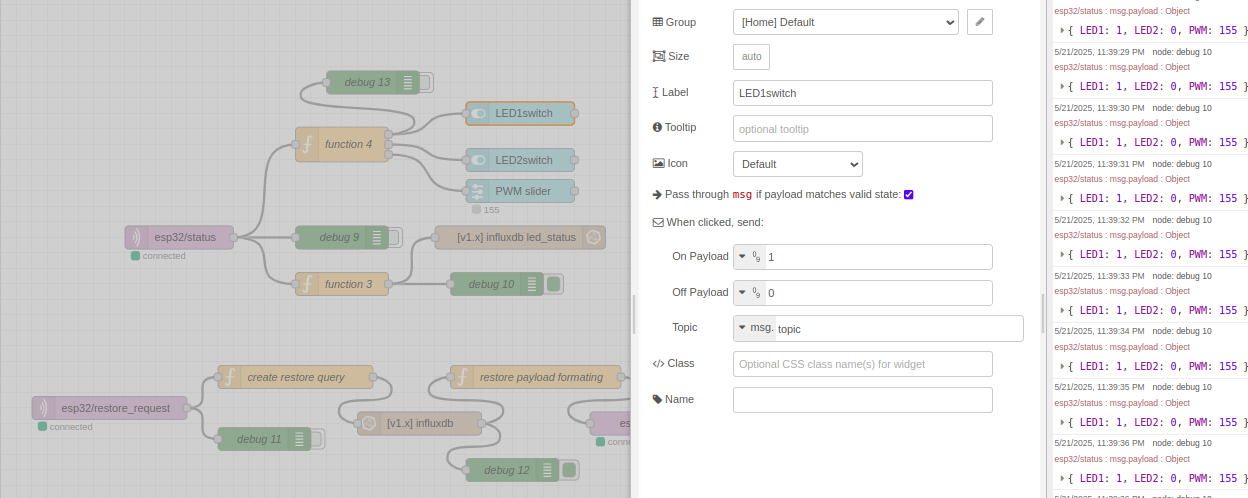
\includegraphics[width=0.9\textwidth]{ui_conf.png}
			\caption{configuration show for slider of led1.}
			\label{fig1:}
		\end{figure}		

	
	A screenshot of the visualization is presented below, having the 2 switches and the slider,
	and for debug purposes the plots of the incoming data from accelerometer and gyrometer.

		\begin{figure}[H]
			\centering
			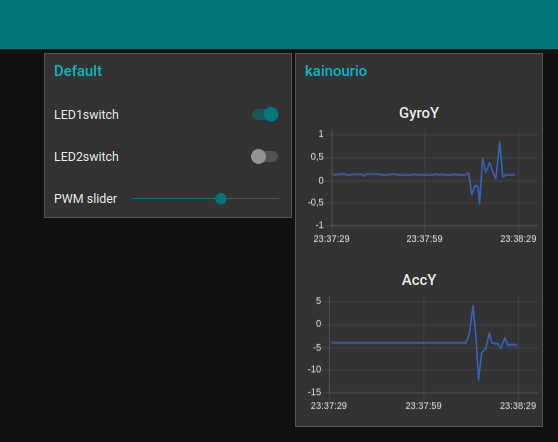
\includegraphics[width=0.9\textwidth]{ui_threshold.png}
			\caption{Node-Red UI.}
			\label{fig1:}
		\end{figure}		


\section{Summary of Data Flow}

\begin{center}
\begin{tabular}{|l|l|l|}
\hline
\textbf{Component} & \textbf{Topic / Action} & \textbf{Description} \\
\hline
ESP32 & Publish \texttt{esp32/restore\_request} & Sends \texttt{get\_latest} on startup \\
Node-RED & MQTT In on \texttt{esp32/restore\_request} & Detects restore request \\
Node-RED & InfluxDB query & Fetch last saved LED/PWM states \\
Node-RED & Function node & Format restore state payload \\
Node-RED & MQTT Out on \texttt{esp32/restore\_state} & Publishes restore state \\
ESP32 & MQTT Subscribe \texttt{esp32/restore\_state} & Receives and applies restore state \\
ESP32 & Publish \texttt{esp32/status} & Periodic status updates \\
\hline
\end{tabular}
\end{center}



\section{Motion detection via machine learning}

In the second part, the goal is to move from the threshold supported movement detection and achieve the 
operational functionalities by employing machine learning. Communication with Node-Red remains 
the same, as the machine learning classifier is executing only in ESP32 having as a result the usage
of the same topics and the same integration across ESP32-NodeRed.

\subsection{Data acquisition}

For data acquisition for each gesture, \texttt{mpu\_record.py} have been utilized in
order to send over UART a message "record" and then create samples for each of the two
classifiers respectively.
After manually we create the appropriate files to pass in the Python scripts to generate the
C functions to be used in ESP32 and use the trained classifiers.




\subsection{LEDs activation}
The system in this configuration uses the readings from the MPU9250 IMU 
and machine learning to control the LEDs. For the data collection and feature processing the IMU
continuously reads acceleration (ay) and gyroscope (gy) 
data along the Y-axis. These values are stored in an implemented circular buffer (featureBuffer)(CircularBuffer.h)
that maintains the 20 most recent samples(10 measurements of each Y axis of accelerometer and gyroscope)

When the buffer is full (20 samples), the features 
are processed for classification.
The raw features are first scaled using the StandardScaler parameters which were generated on the \texttt{micro2.py} Python training script
(scaler\_mean and scaler\_scale). The system then calculates Euclidean distances 
between the current scaled features and three reference scaled patterns (LED1, LED2, and Neutral) as a similarity measure.
If the distance to the Neutral pattern is below 2.0, our implemented system 
considers it a neutral position and takes no action

Otherwise if any of the euclidean distances between the current stored sample and the three classes(LED1 TOGGLE,LED2 TOGGLE and NEUTRAL), 
the features are passed to the SVM classifier (trained in \texttt{micro2.py} 
which predicts whether the motion corresponds to LED1 toggle, LED2 toggle, or Neutral.
When a "LED1\_TOGGLE" prediction is made, 
and at least 900ms have passed since the last toggle (debouncing method).
The led1State boolean is flipped (true to false or false to true)
The PWM duty cycle is set to pwmLevel variable if ON, or 0 if OFF.
Same logic as LED1, is followed for controlling "LED2\_TOGGLE" prediction.

If confidence is below 75\%, the system falls back 
into using just the distance metrics for classification.
As an addition the 900ms delay between toggles is used in order to prevent 
rapid accidental toggling that can occur inside the same running sliding window as
traversing the circular buffer of features.
Also the confidence threshold helps for filtering out uncertain predictions.

The SVM classifier used for the LEDs activation and determining actions as LED1\_TOGGLE, NEUTRAL and LED2\_TOGGLE
is getting as an input 20 features which consist of 10 samples of continuous values of (ay,gy) : 
\newline 
(\textit{ay1,gy1,ay2,gy2,...ay10,gy10}).

\begin{figure}[h!]
\centering
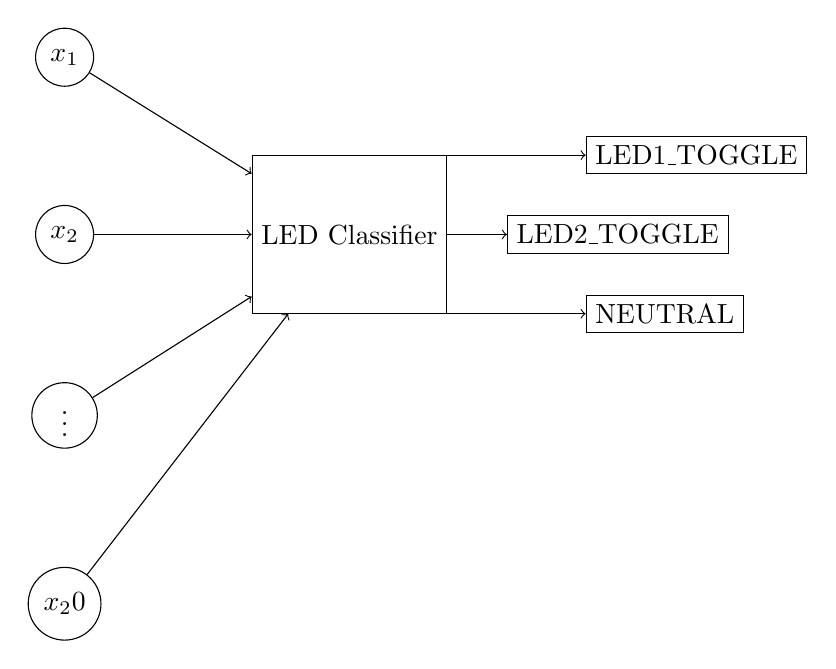
\begin{tikzpicture}[node distance=1.5cm and 2cm, auto]

% Input nodes
\node[draw, circle] (x1) {$x_1$};
\node[draw, circle, below=of x1] (x2) {$x_2$};
\node[draw, circle, below=of x2] (x3) {$\vdots$};
\node[draw, circle, below=of x3] (xn) {$x_20$};

% SVM box
\node[draw, rectangle, right=2cm of x2, align=center, minimum height=2cm, minimum width=2cm] (svm) {LED Classifier};

% Output nodes
\node[draw, rectangle, right=3cm of svm.north] (y1) {LED1\_TOGGLE};
\node[draw, rectangle, right=2cm of svm.center] (y2) {LED2\_TOGGLE};
\node[draw, rectangle, right=3cm of svm.south] (y3) {NEUTRAL};

% Connections
\foreach \i in {x1,x2,x3,xn}
    \draw[->] (\i) -- (svm);

\draw[->] (svm.north east) -- (y1);
\draw[->] (svm.east) -- (y2);
\draw[->] (svm.south east) -- (y3);
\end{tikzpicture}
\caption{The SVM classifier used for the LED activation actions.}
\end{figure}






\subsection{Control of PWM}

For controlling the common PWM applied in each LED in case it is "ON",
we create a second classifier which works with data acquired from 
magnetometer X axis readings. 

The SVM classifier used for determining the increase/decrease of the global used PWM value
is getting as an input 9 features which consist of 9 samples of continuous values of (mx) : 
\newline 
(\textit{mx1,mx2,...mx9}).

\begin{figure}[h!]
\centering
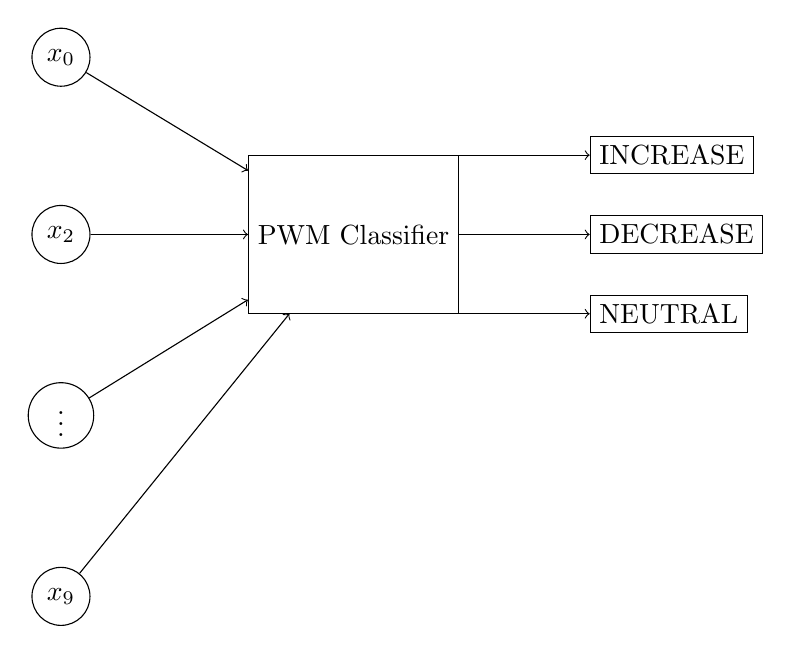
\begin{tikzpicture}[node distance=1.5cm and 2cm, auto]

% Input nodes
\node[draw, circle] (x1) {$x_0$};
\node[draw, circle, below=of x1] (x2) {$x_2$};
\node[draw, circle, below=of x2] (x3) {$\vdots$};
\node[draw, circle, below=of x3] (xn) {$x_9$};

% SVM box
\node[draw, rectangle, right=2cm of x2, align=center, minimum height=2cm, minimum width=2cm] (svm) {PWM Classifier};

% Output nodes
\node[draw, rectangle, right=3cm of svm.north] (y1) {INCREASE};
\node[draw, rectangle, right=3cm of svm.center] (y2) {DECREASE};
\node[draw, rectangle, right=3cm of svm.south] (y3) {NEUTRAL};

% Connections
\foreach \i in {x1,x2,x3,xn}
    \draw[->] (\i) -- (svm);
\draw[->] (svm.north east) -- (y1);
\draw[->] (svm.east) -- (y2);
\draw[->] (svm.south east) -- (y3);
\end{tikzpicture}
\caption{The SVM classifier used for the PWM actions.}
\end{figure}



	\subsubsection{Classifier's training and integration with the ESP32 platform.}
	Both of the SVM classifiers are trained in a local host with higher computational capabilities than ESP32, 
	in order to achieve classification accuracy and then transfer in the embedded system only the libraries 
	which include the weights of the trained classifier.  After generating both of the classifiers their respective library 
	files PWMClassifier.h and LEDClassifier.h are included in the source file which will be compiled and uploaded to the ESP32.
	In the source files the training for both is implemented in \texttt{micro2.py,micro3.py} respectively. Also in these files
	after training we do create one reference average sample per class which later is used for similarity comparison in the ESP32.


	\paragraph{Why euclidean distance was chosen over cosine similarity:}

	When detecting the class closest to a given point in feature space, 
	Euclidean distance can be more appropriate than cosine similarity in situations 
	where the absolute proximity of the vectors is more important than their directional alignment. 
	While cosine similarity measures how aligned two vectors are (ignoring magnitude), 
	Euclidean distance accounts for both the direction and the magnitude. 
	This becomes crucial in our situation as well as shown experimentaly from the data, 
	where cosine similarity was shown better similary to wrong gesture because the sample of 
	the wrong class was an amplification of the correct's one.
	Its like in a graphical space  when one class is slightly rotated or "hidden behind" 
	another in angle they may have different orientations but still be physically close in space. 
	In such cases, cosine similarity might consider them very different due to the angle, 
	even though they are spatially close. 
	Euclidean distance, in the other hand would correctly reflect their true closeness, 
	making it better suited for identifying the nearest class based on actual position rather than orientation.	
	For this reason in this project Euclidean distance has been utilized over the cosine similarity as a similarity measure.


	A screenshot is presented also which shows both classifiers classifying the gesture as to increase the PWM which is applied on
	the LEDs and with the LED2 toggled. We can observe the classification outputs and also the Euclidean distances for each sample
	against the reference scaled average vectors who describe each class.

	\begin{figure}[H]
			\centering
			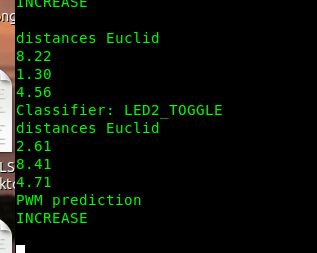
\includegraphics[width=0.9\textwidth]{classification.png}
			\caption{classification screenshot.}
			\label{fig1:}
		\end{figure}		




	From out terminal also we can observe the values inside our esp32db database in \texttt{led\_status} measurements.c
	There is timestamp, led1 status(0-off 1-on), led2 status(same as led1) and the common pwm value.
	\begin{figure}[H]
			\centering
			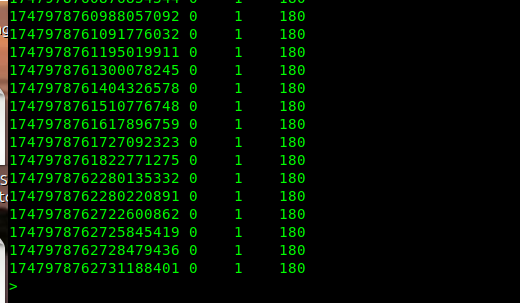
\includegraphics[width=0.9\textwidth]{influx.png}
			\caption{Querying our esp32db: select * from led\_status}
			\label{fig1:}
		\end{figure}		

\end{document}

